\chapter{序論}
\label{chap_intro}
\newpage

\section{研究背景}
\subsection{福祉ロボット}


\subsection{ロボットのメカやソフトの進歩}
ロボティクス技術の向上とともに,様々な分野でロボットが活躍している.特に,医療や福祉といった人間の生活環境下で作業可能なパーソナルロボットの需要の増加は顕著である.しかし,人の生活環境下において完全に自律して動作及び人の補助ができるロボットの実現は困難な状況にある.なぜならば,ロボットが自律行動を行うためには物体や人物の認識,自己位置の認識,そして認識に基づく判断を人の生活環境下で行わなければならないからである.

パーソナルロボットとしてMobile Manipulatorの開発が行われている.Mobile Manipulatorは工場に限定されて使用されているが,これを家庭内でも使用できるように軽く,そして小さくすることで衝突リスクを削減する試みがされている.2018年には,Preferred Networksは室内に散らかった家庭用品を片付けるロボットシステムを発表した\cite{お片づけロボット}.部屋の全自動片付けは従来のロボットシステムでは実現困難であったが,近年の深層学習の発展によって初めて実用的なレベルとなった.物をつかむ,物を置く,動作計画を立てる,人の指示に対応するなど,ロボットが人間の生活空間で仕事をするために必要な物体認識・ロボット制御・音声言語理解技術に最先端の深層学習を用いた結果,ロボットが高速・高精度に動作できるようになった.

しかし,深層学習では多くの計算リソースが必要である.計算リソースとは深層学習を動かすハードウェア(いわゆるPC),特にGPU(Graphical Processor Unit)である.GPUは形状が大きく消費電力も大きいため,高性能なGPUを複数Mobile Manipulatorに搭載することは難しい.そこでCloudネットワークを利用する方法がある.Cloudを介してGPUリソースを使用する.これによりCloudとのインターフェースを有しているデバイスであれば演算性能は低くても推論が可能となり,スマートフォンやノートPC,ラズパイと言った小さなデバイスを使用することができる.しかし常時インターネットに接続している必要があるため,災害時に使用できなくなるという問題がある.一方で,Cloudを使わずLocalで処理を行うEdgeコンピューティングという分野も近年研究開発がされている.Edgeコンピューティングでは一般のPCに搭載するようなGPUを用いず,より小型なデバイス(エッジデバイス)で処理を行うことを目的としており,小型,低消費電力,高精度より高速が求められる.しかし深層学習を使用しているパーソナルロボットは高さ1 mと大きく重量も大きいため誤動作時のリスクが大きい.また,家庭内などで使用する分には良いが外に持ち出してどこでも使用するといった事ができない.


\subsection{医療分野における電動義手}
医療分野におけるロボットの用途として期待されるものと言えば電動義手である.義手には装飾用義手や能動義手,作業用義手などがあるが,現在主流の筋電電動義手(筋電義手)は,使用者が筋肉を動かすことで筋電位を読み取り直感的な操作を可能にする.しかし,筋電位を用いた義手には訓練が必要でリハビリテーション施設で行う必要があるが,その施設が極めて少ない\cite{リハビリテーション}.また筋電位が上手く出せない患者や,腕そのものはあるが麻痺して動かせない患者に対しては使用できない.さらに非侵襲的な筋電義手では入力信号が限られる.自由度の高い動作を可能にする電動義手は重量が大きくなり,使用者の負担が大きくなってしまう.

筆者は茨城県立医療大学付属病院リハビリテーション科にて義手使用患者へのヒアリングを実施した.
当患者は日常では能動義手を使用しており,病院でのリハビリの際に筋電義手の使用訓練を行なっている.半年のリハビリの後,ようやくペンを掴むことまでできた状況とのこと.筋電義手の使用感については,
\begin{itemize}
    \item "筋電義手は重い."
    \item "(筋電が)ちゃんと伝わっているかわからない."
    \item "把持力の制御が難しく,(物を)落とすこともよくある."
\end{itemize}
とあまりポジティブな感想はなかった.ヒアリングを通して得た課題をまとめると,
\begin{itemize}
    \item 義手本体が重い
    \item 筋電による義手の制御が難しい
    \item リハビリは大変で多くの時間を要する(割にはできる動作は把持のみ)
\end{itemize}
である.以上のような課題があるため装着者のニーズを満たす義手がなく,実用化に至っていないのが現状である.

% 重量の重要性を書く

\section{関連研究}
ここでは近年の福祉ロボットの研究について紹介する.

TOYOTAは障がい者や高齢者などの家庭内での自立生活をアシストする生活支援ロボットHSR(Human Support Robot)を開発した\cite{HSR2019}.
\begin{figure}[H]
    \centering
    \begin{minipage}{0.6\hsize}
        \centering
        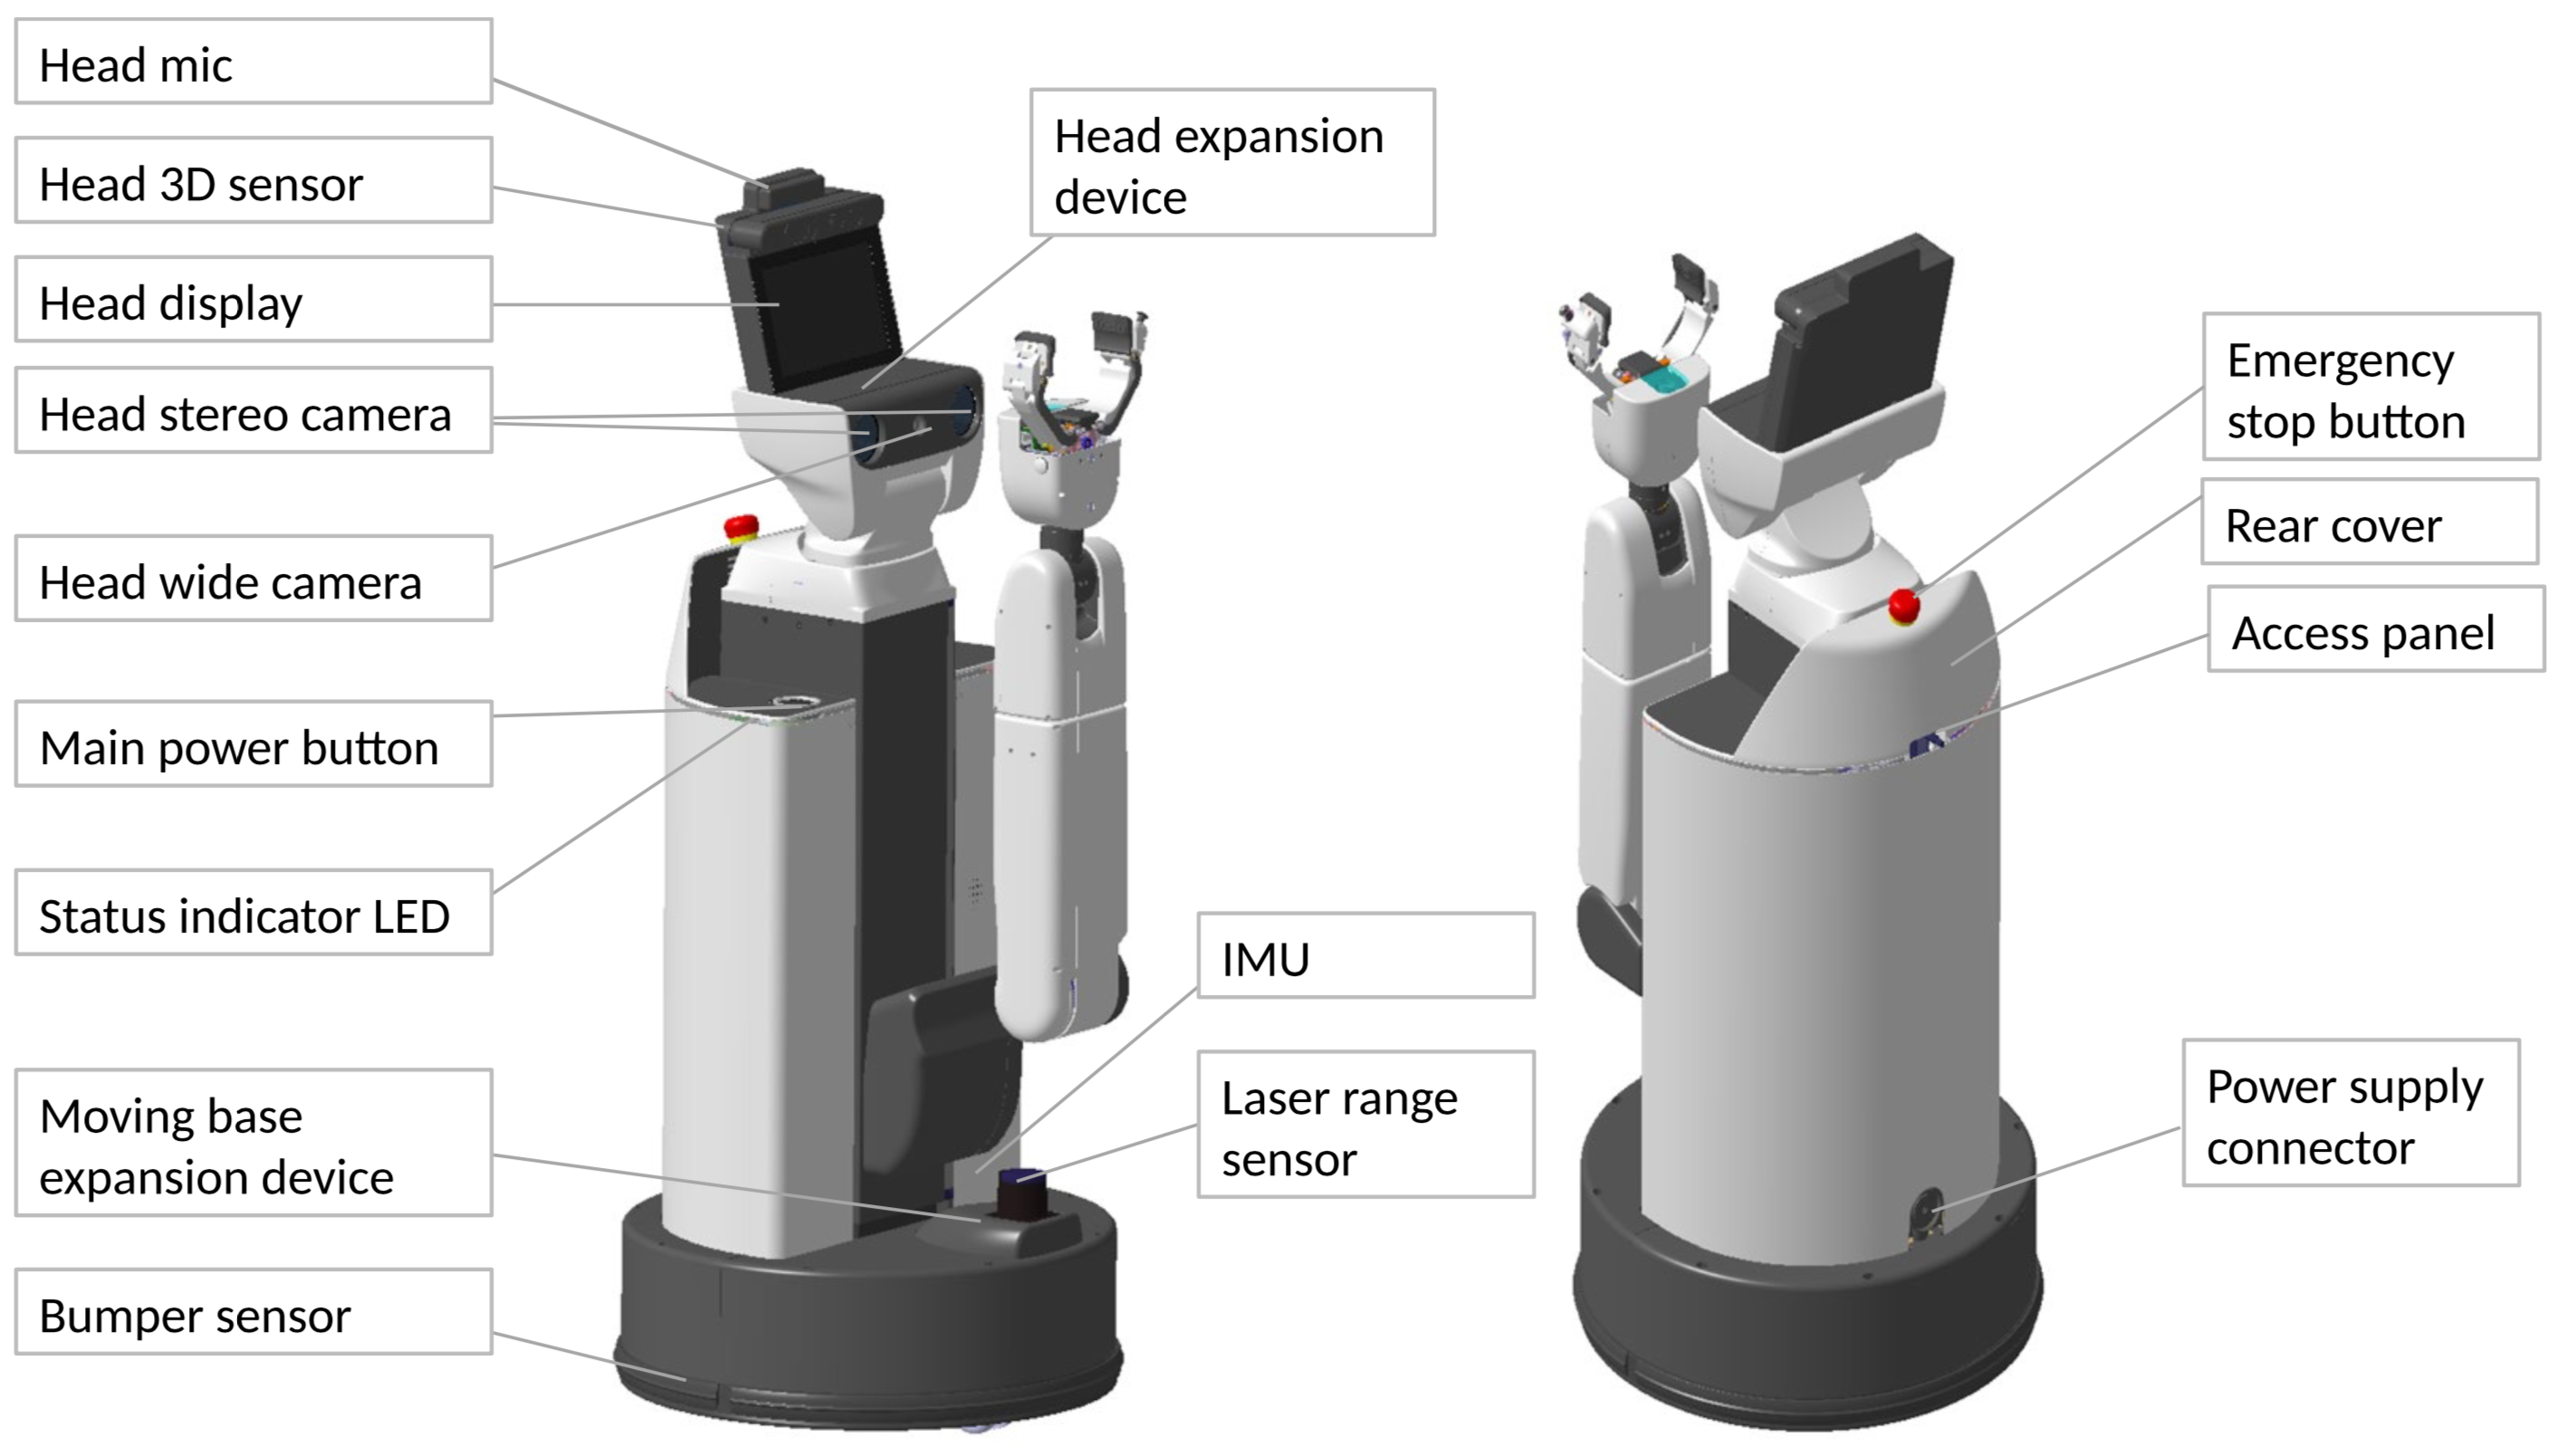
\includegraphics[width=\linewidth]{figure/chapter1/HSR_paper-2}
    \end{minipage}
    \begin{minipage}{0.39\hsize}
        \centering
        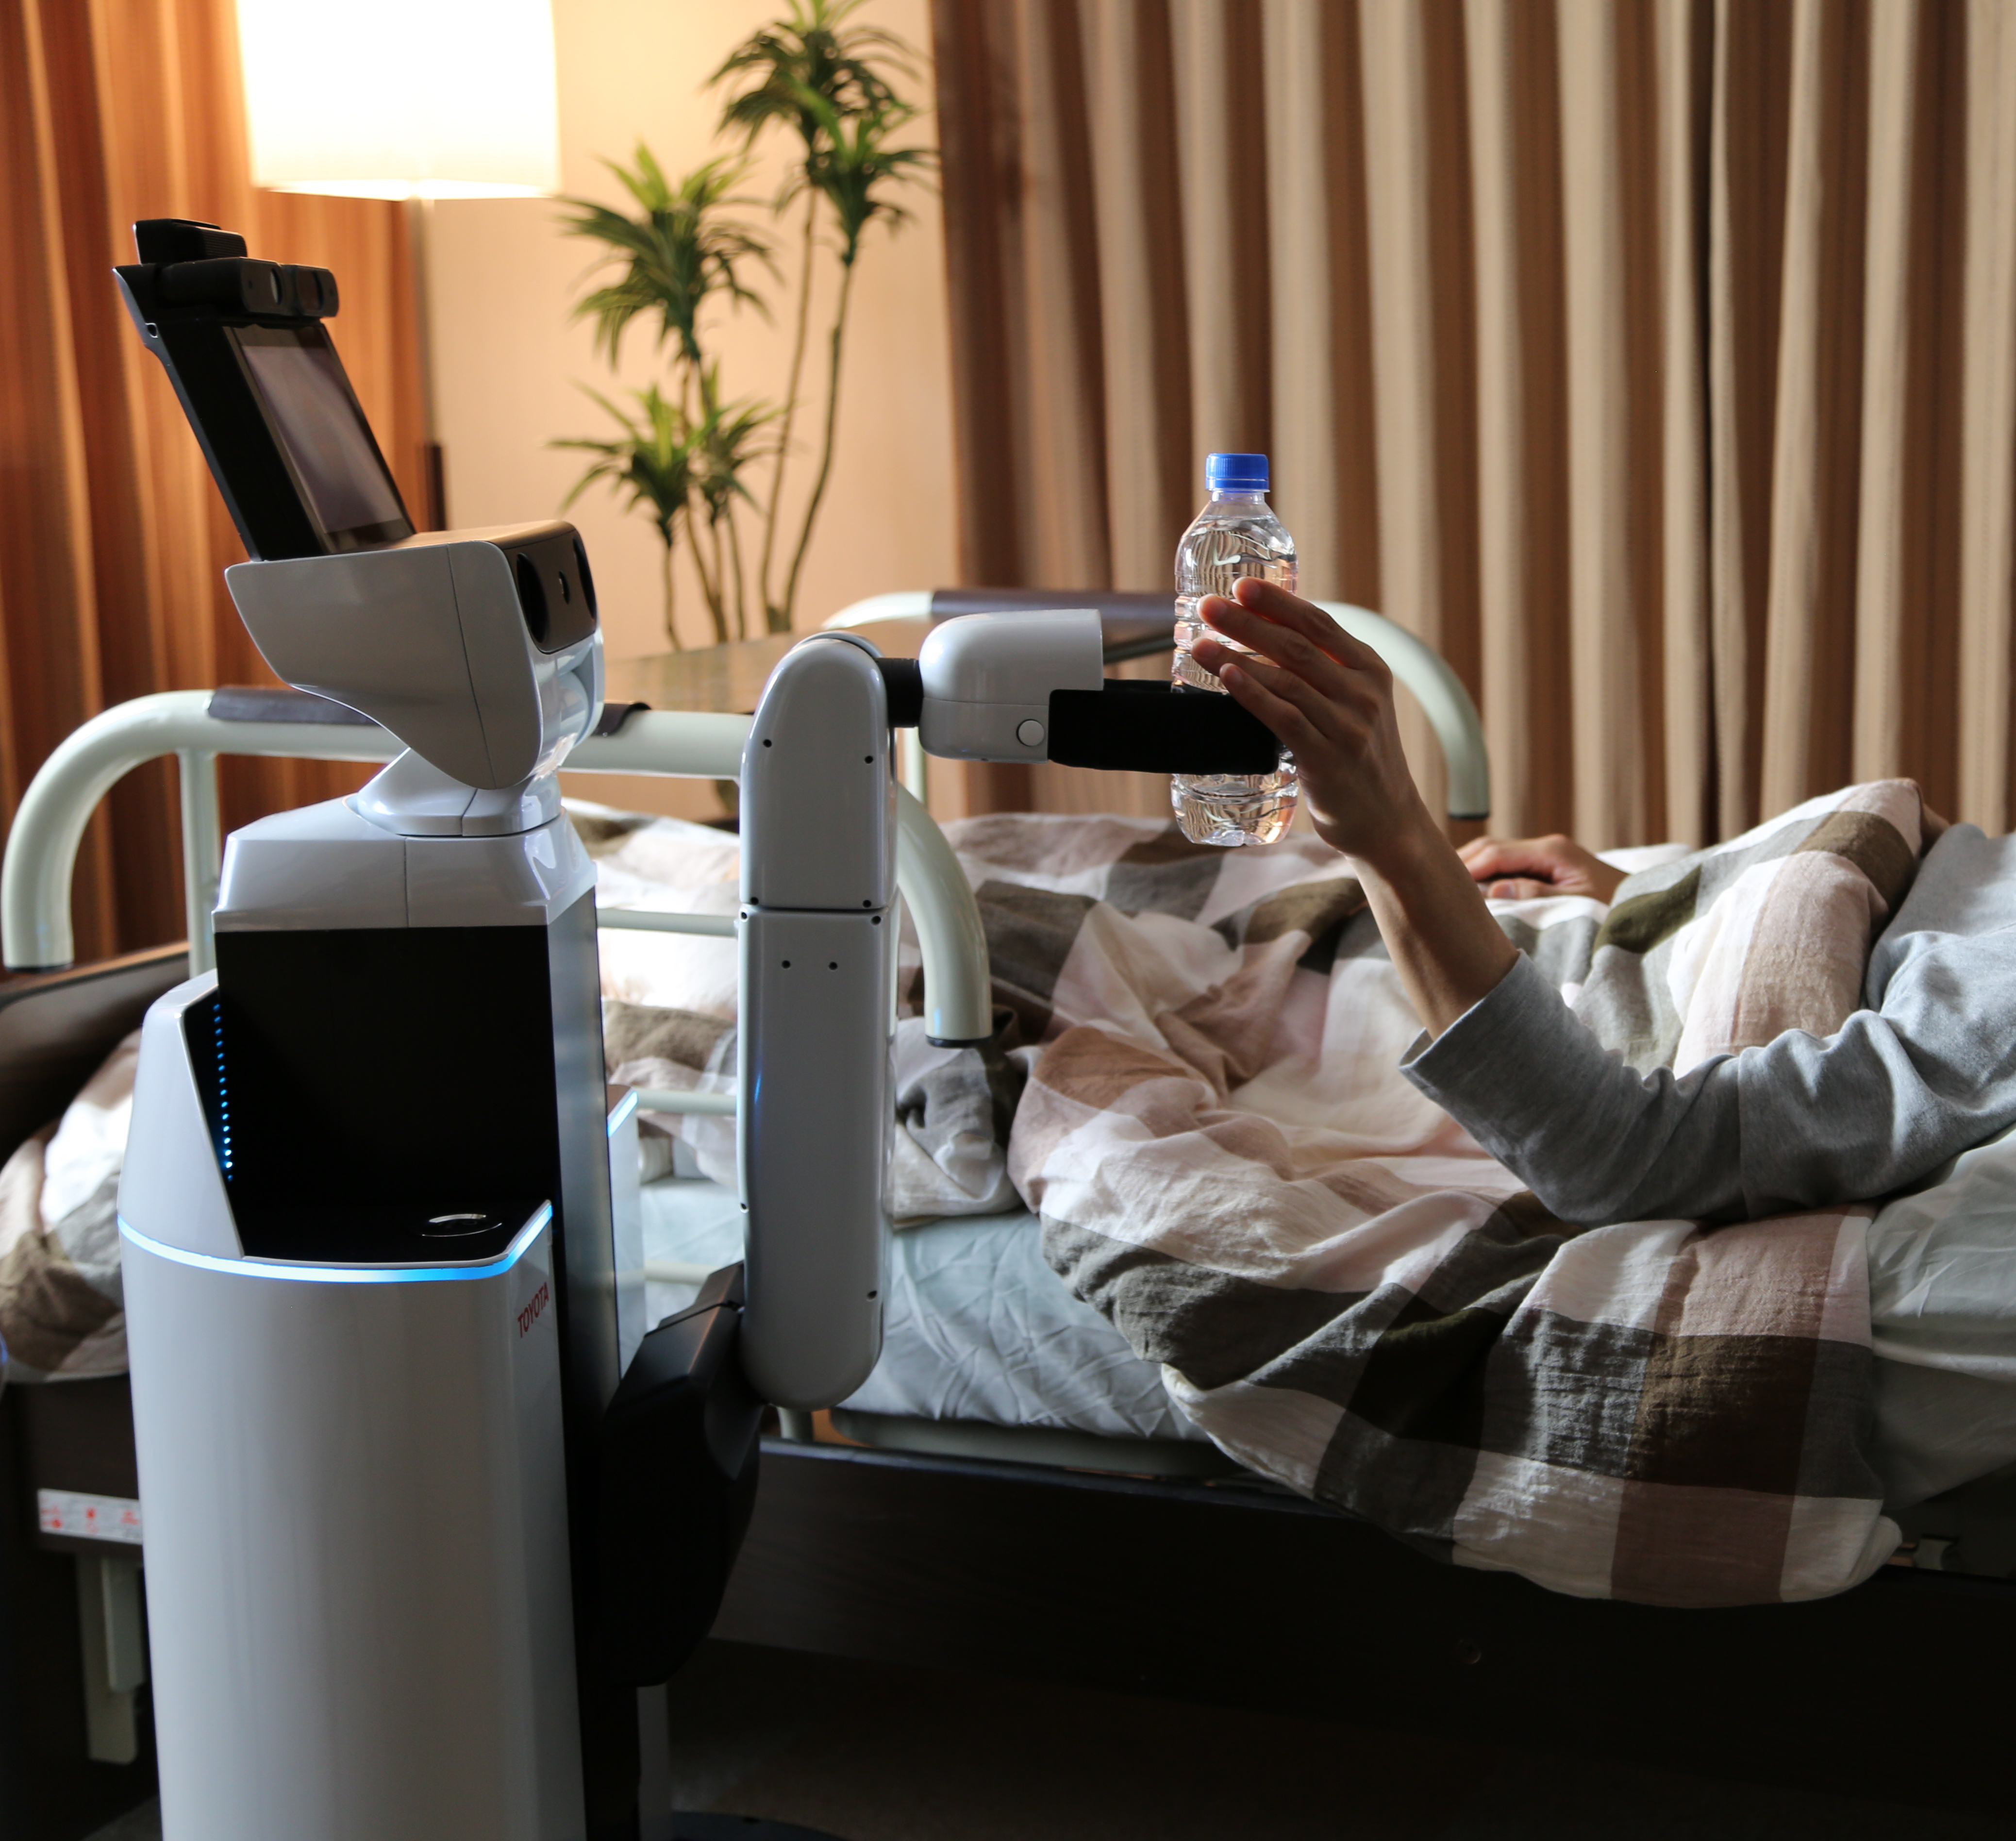
\includegraphics[width=\linewidth]{figure/chapter1/HSR_site-2}
    \end{minipage}
    \caption[Human Support Robot (HSR) produced by TOYOTA.]{Human Support Robot (HSR) produced by TOYOTA\cite{HSR2018, HSRサイト}.}
    \label{fig:HSR}
\end{figure}


筑波大の山海グループは片麻痺患者の日常生活を支援するサイバニックロボットアームを開発した\cite{Sankai2018}.片麻痺者の失われた上肢機能を代替可能なロボットアームを研究開発し,片麻痺者が上肢作業に抱える問題を解決することを目的としています.健常な手・腕の生体情報の活用や知能化・自動化によりロボットアームをサイバニック化することで,あたかも使用者の腕であるかのように人の意思に基づいて機能するサイバニックロボットアームの実現を目指しています.
\begin{figure}[H]
    \centering
    \begin{minipage}{0.49\hsize}
        \centering
        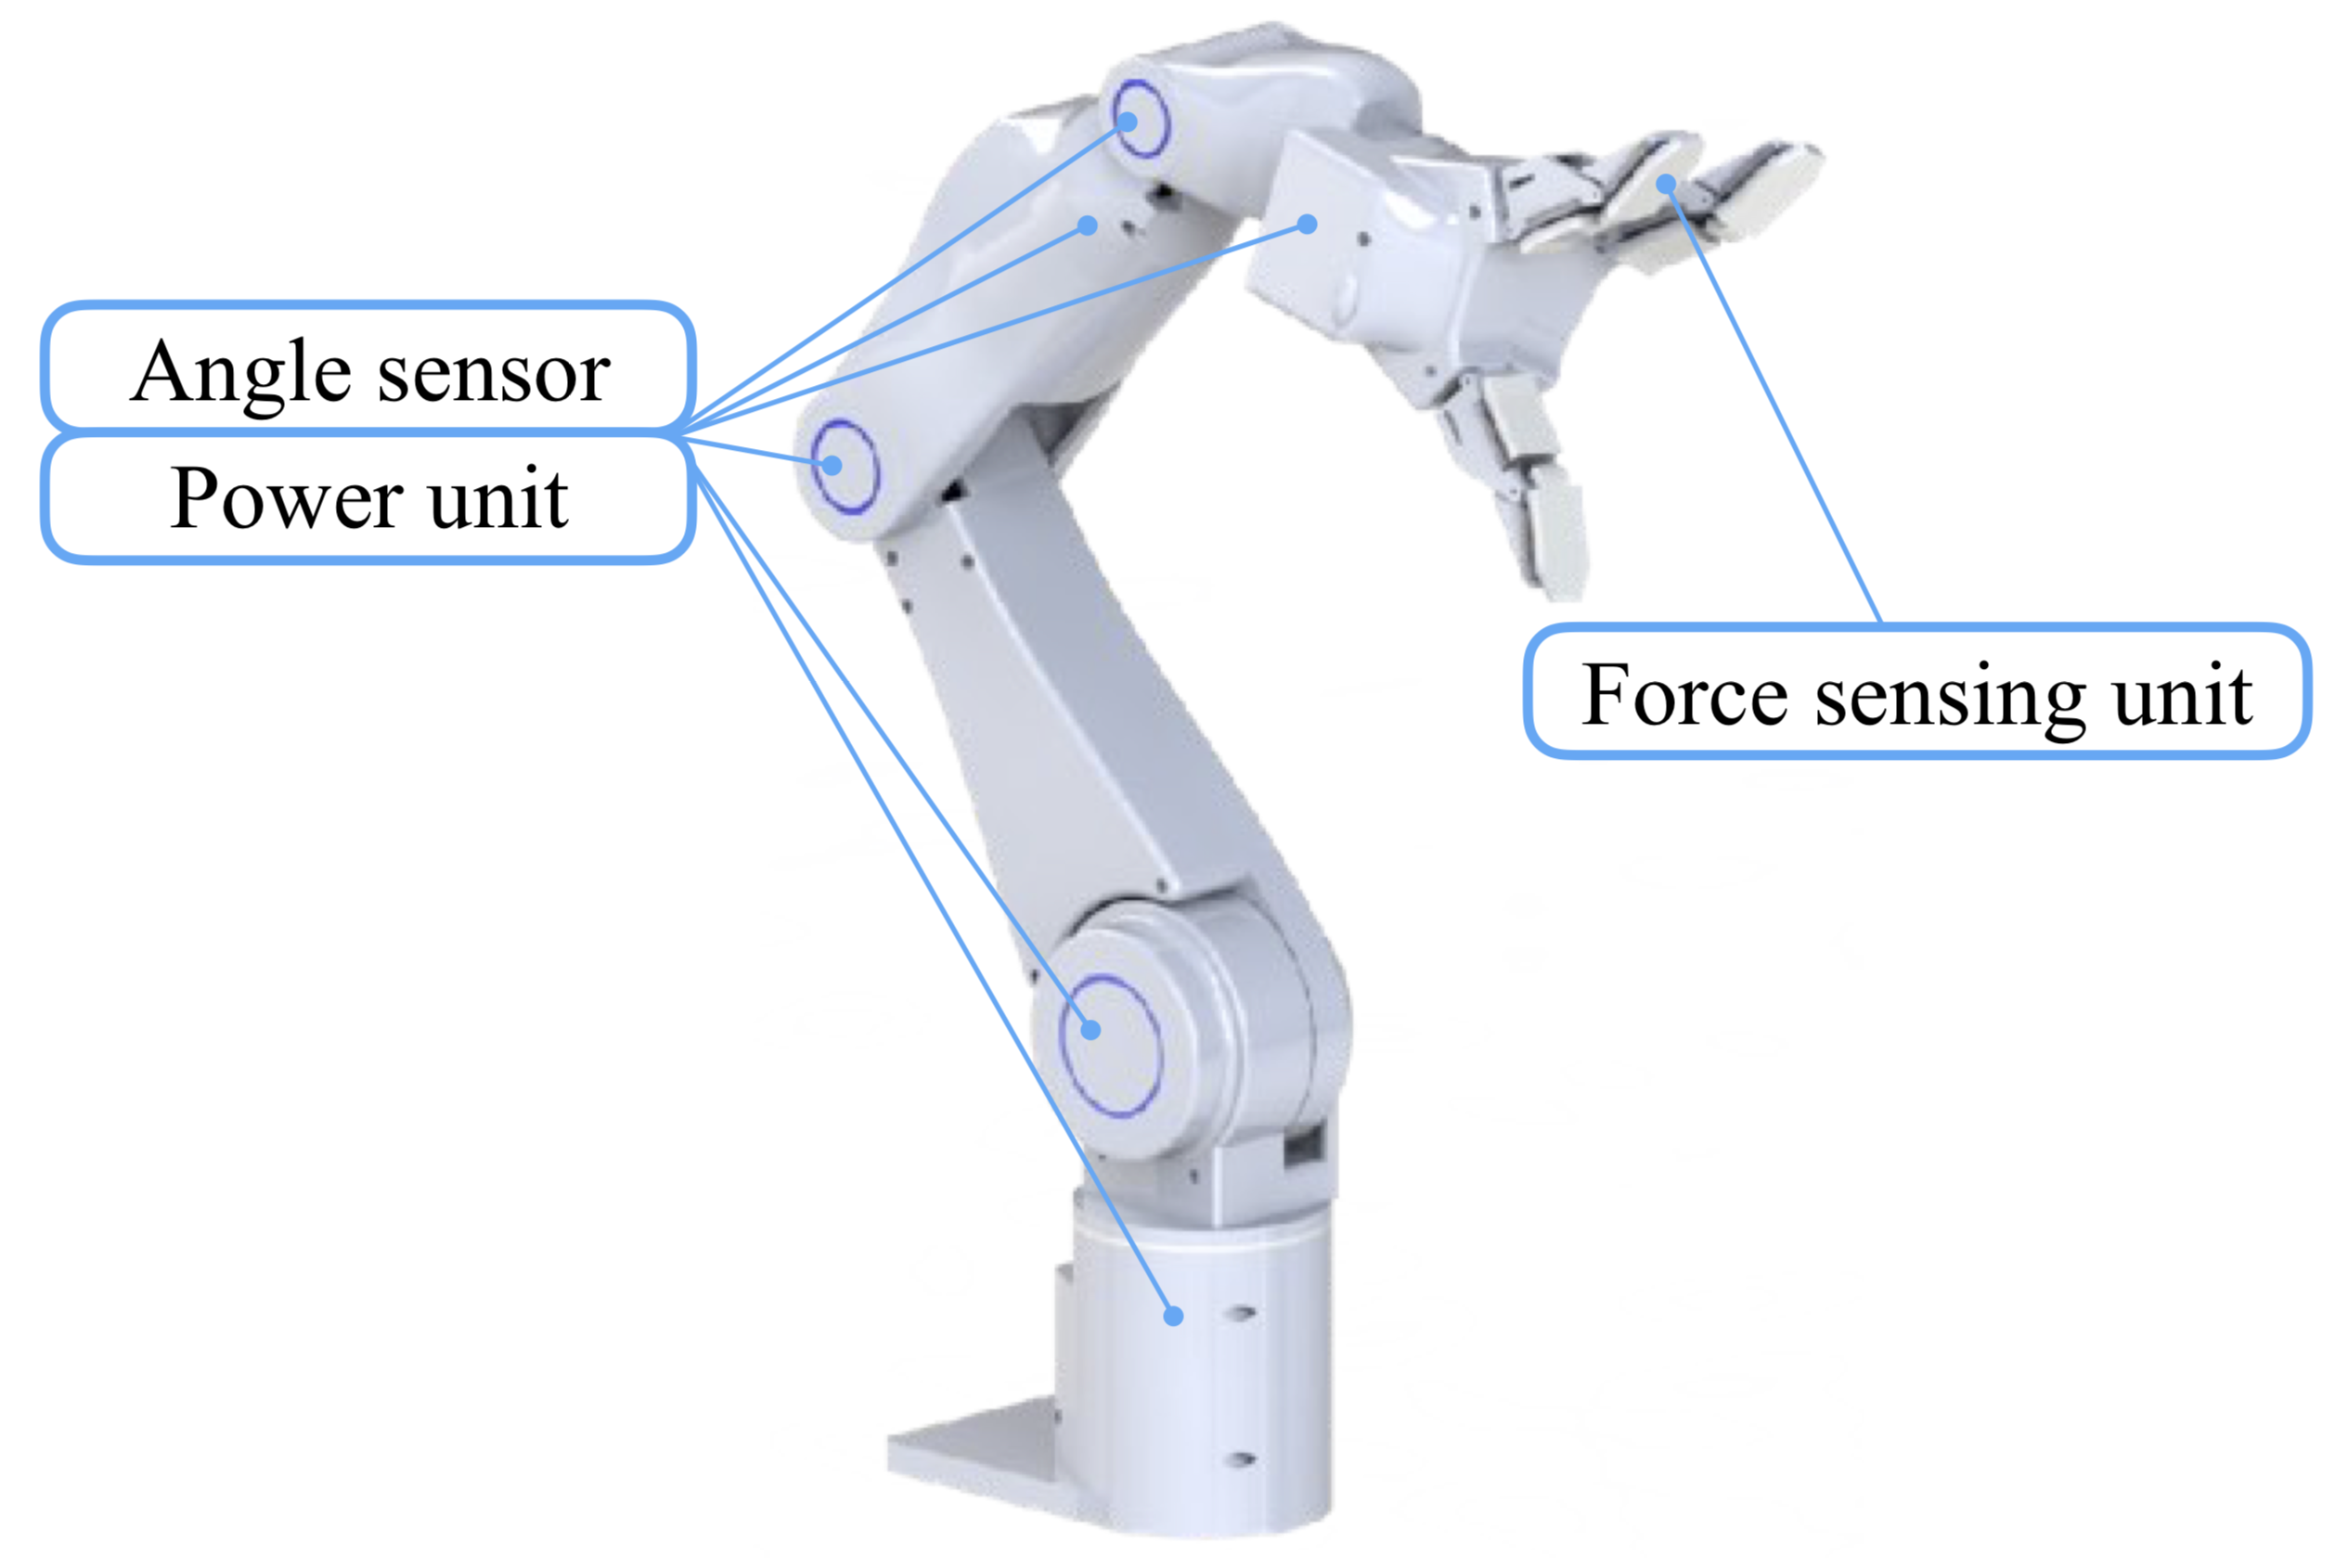
\includegraphics[width=\linewidth]{figure/chapter1/cybernic_arm_2017-2}
    \end{minipage}
    \begin{minipage}{0.49\hsize}
        \centering
        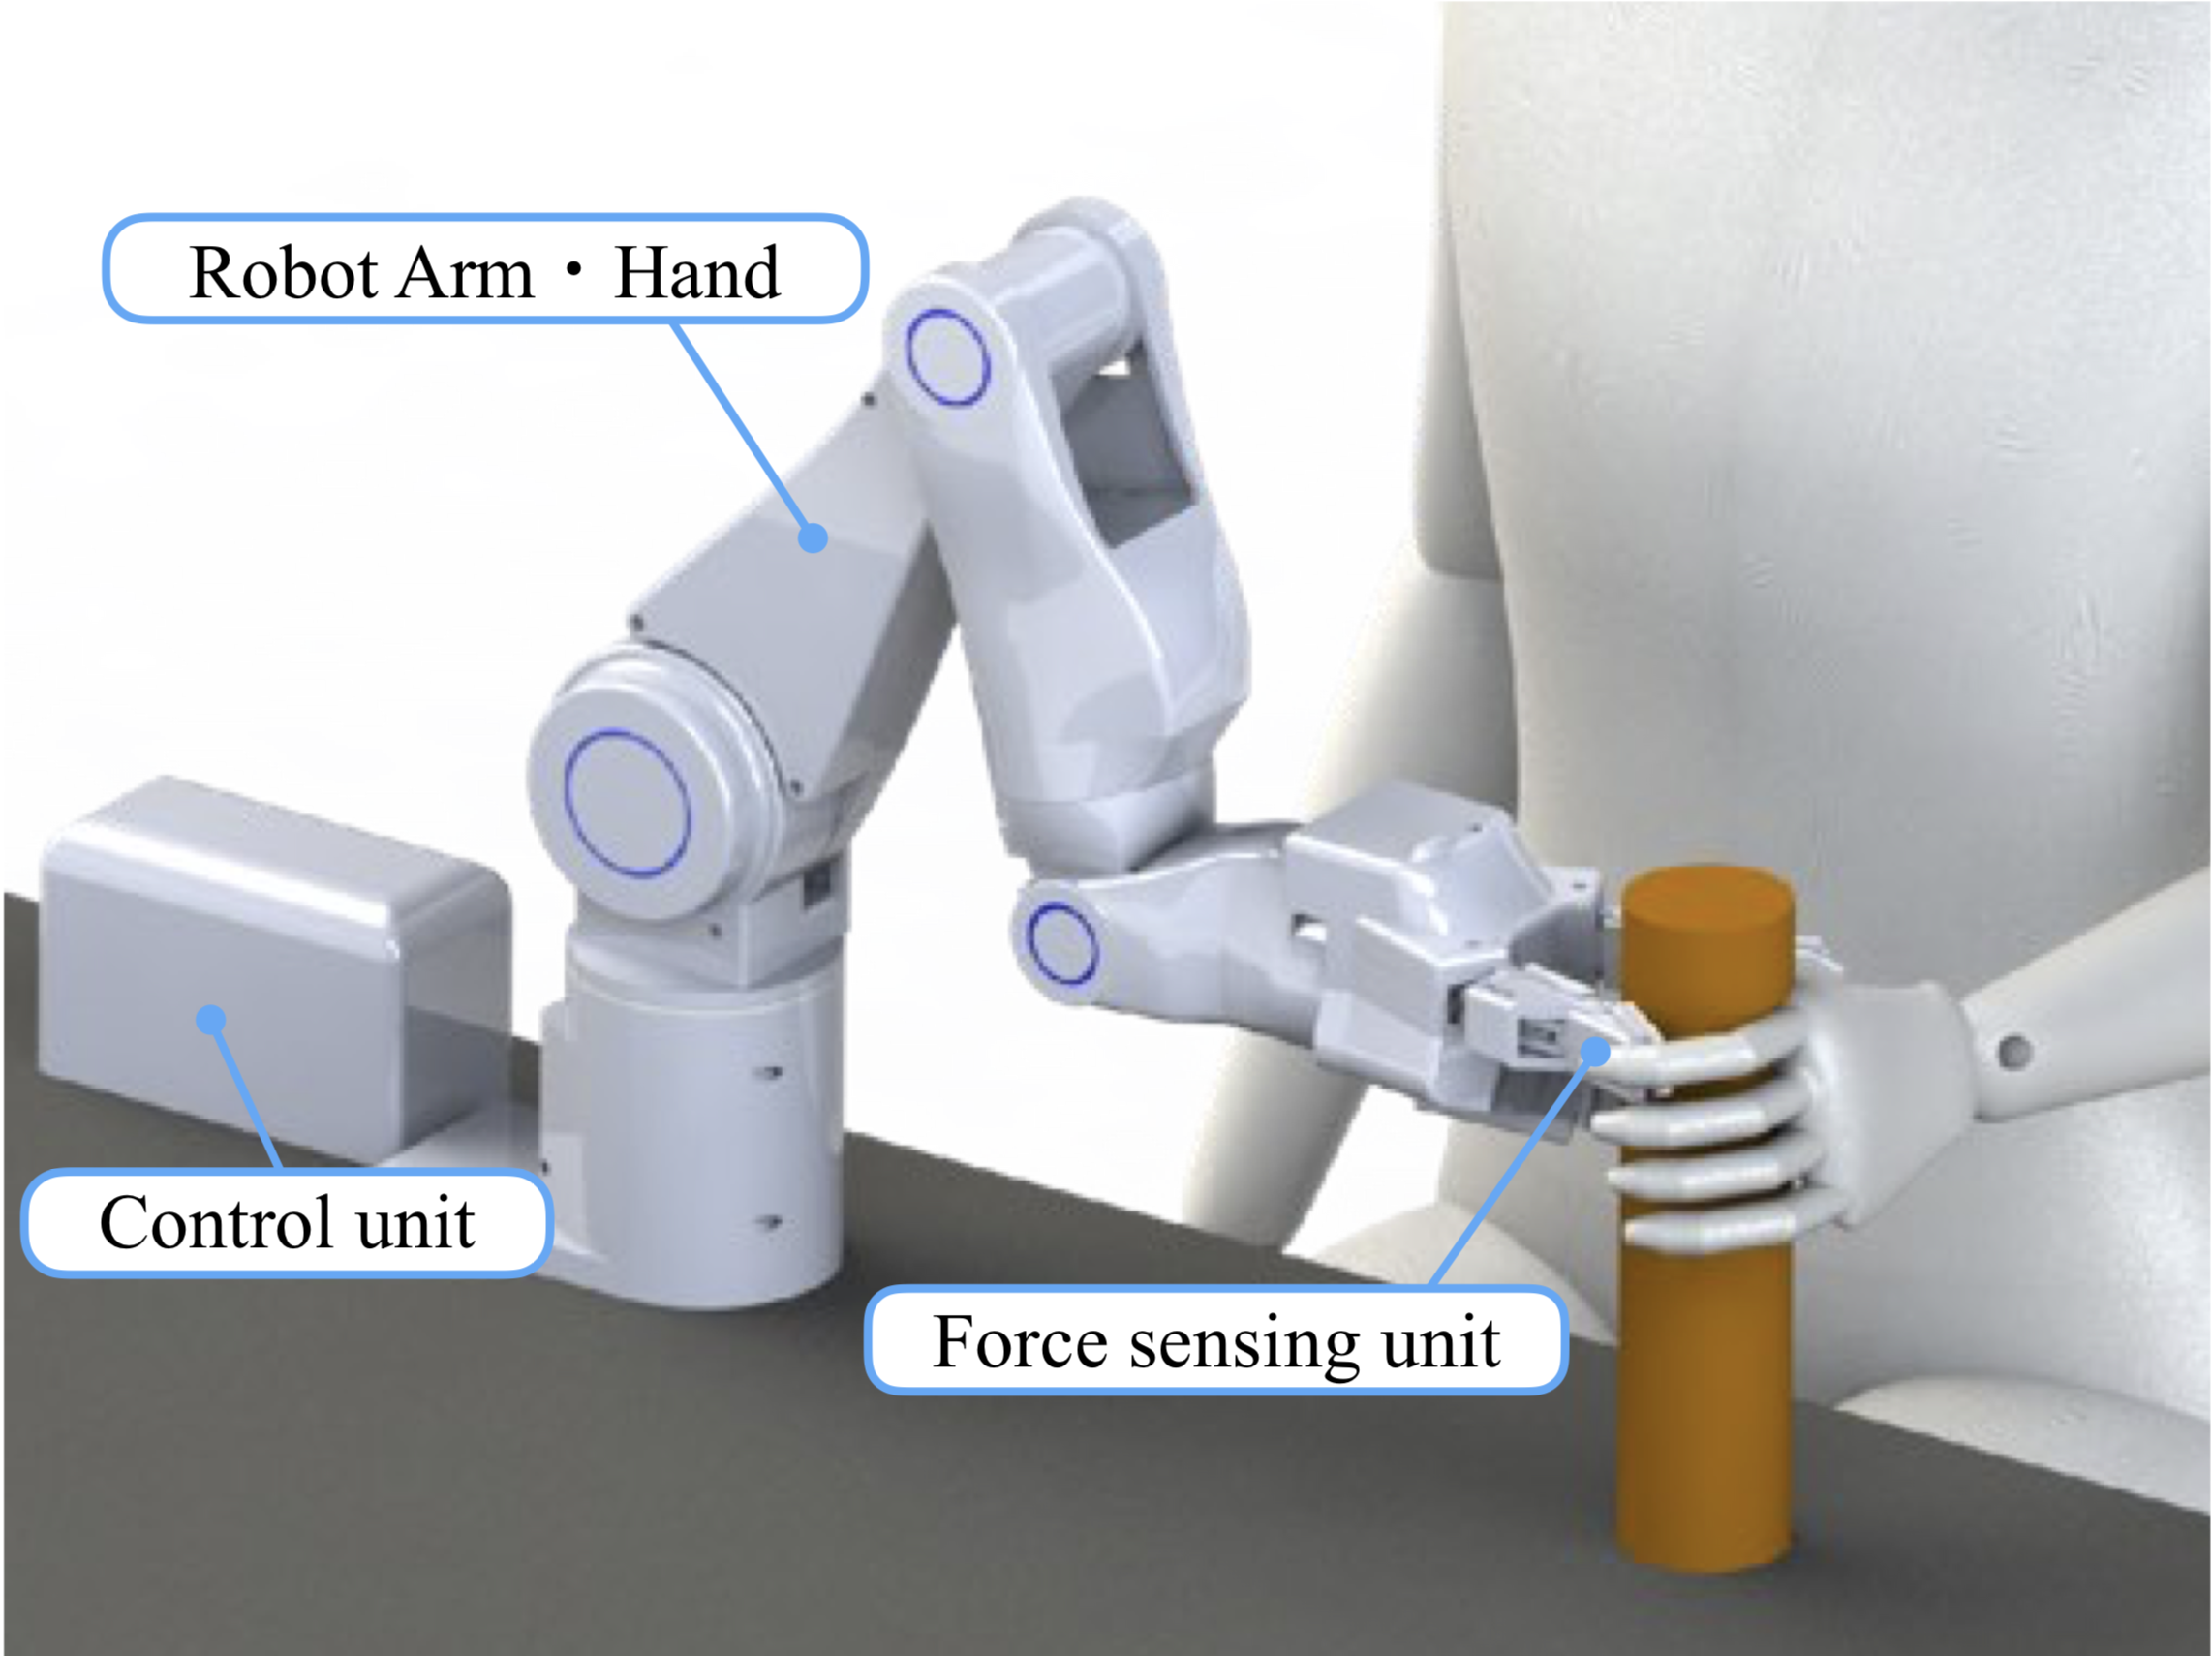
\includegraphics[width=\linewidth]{figure/chapter1/cybernic_arm_2017-1}
    \end{minipage}
    \caption[Cybernic robot arm produced by Sankai group.]{Cybernic robot arm produced by Sankai group\cite{Sankai2019}.}
    \label{fig:cybernicarm}
\end{figure}


\section{研究目的}
% 筋電入力を避けた
% 自律走行するロボット
% ニーズを明確化する

本研究ではパーソナルロボットを小型化し,義手使用患者や片麻痺患者など上肢機能障害患者を対象としたパーソナルロボットを開発する.義手は常に身につけているように,パーソナルロボットも携帯できるよう小型化し腕の形をしたロボットハンドとする.上肢機能障害者にとってはパーソナルロボットはどんな事態でも動作する必要があるため,今回はCloudは使用せずEdgeで処理を行うこととする.また座って机で作業することが多いため使用場所を机の上に限定し,指定した物をピックアップするパーソナルロボットハンドを作製することを目的とする.

\section{論文構成}


